%! TEX program = xelatex

\documentclass[10pt]{beamer}

\usepackage[heading = true]{ctex}
% \usepackage[colorlinks,linkcolor=red]{hyperref}

\usepackage{graphicx}
\usepackage{float}
\usepackage{ulem}

\usetheme[]{Boadilla}

\mode<presentation>

\title{
    {自动发帖机器人调研}
}
\author{戴立森}
\date{Nov 10, 2020}

\begin{document}
    \maketitle
    \section*{场景介绍}
        \begin{frame}
            \frametitle{场景介绍}
            \begin{columns}
                \begin{column}{.4\linewidth}
                    国内社交媒体 \\
                    \hspace*{\fill} \\
                    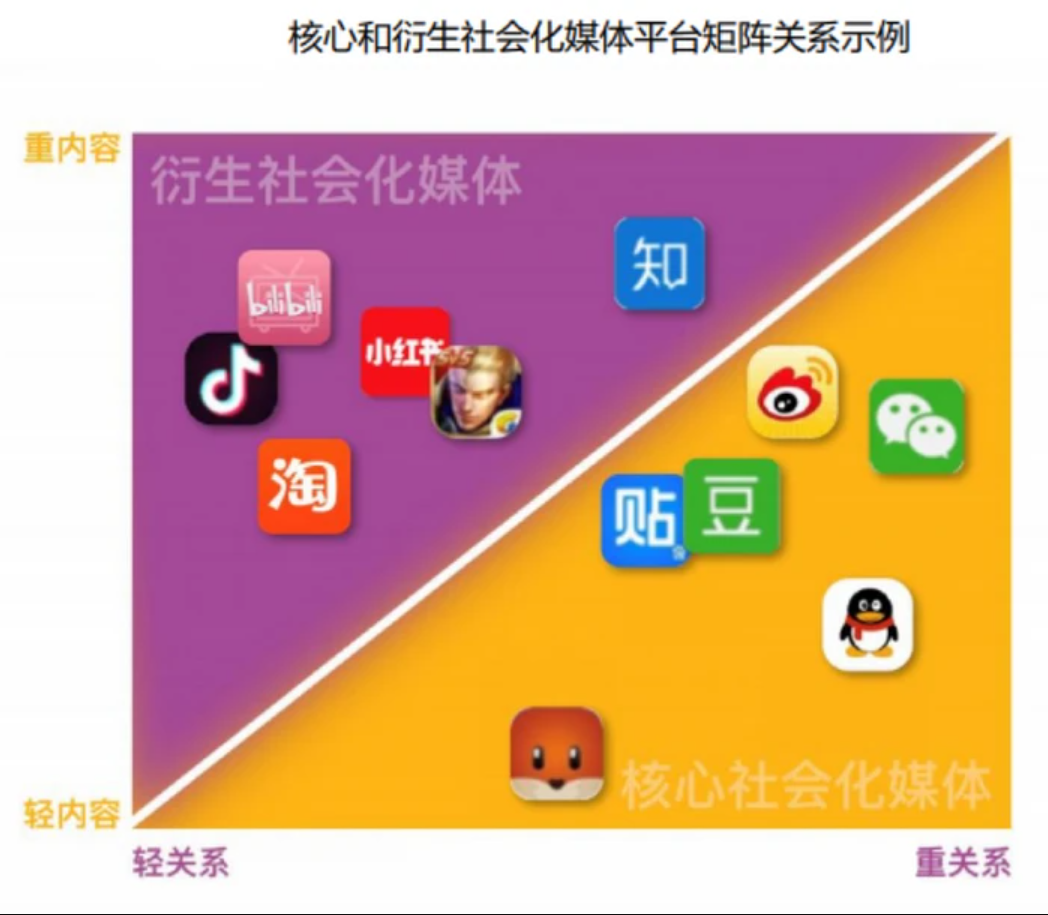
\includegraphics[scale=0.2]{src/img/Social_media_mainland.png}

                \end{column}
                \begin{column}{.4\linewidth}
                    海外社交媒体 \\
                    \hspace*{\fill} \\
                    \hspace*{\fill} \\
                    
\includegraphics[scale=0.07]{src/img/Social_media_oversea.jpg}

                \end{column}
            \end{columns}
        \end{frame}

        \begin{frame}
            \frametitle{场景介绍}
            \begin{columns}
                \begin{column}{.3\linewidth}
                    {\large 一个“帖子”的可能元素} \\
                    \hspace*{\fill} \\
                    \begin{itemize}
                        \item 文字
                        \item 图片
                        \item 短视频
                        \item tag
                        \item 超链接
                        \item ……
                    \end{itemize}

                \end{column}

                \begin{column}{.5\linewidth}
                    
                    \begin{figure}[h]
                        \centering
                        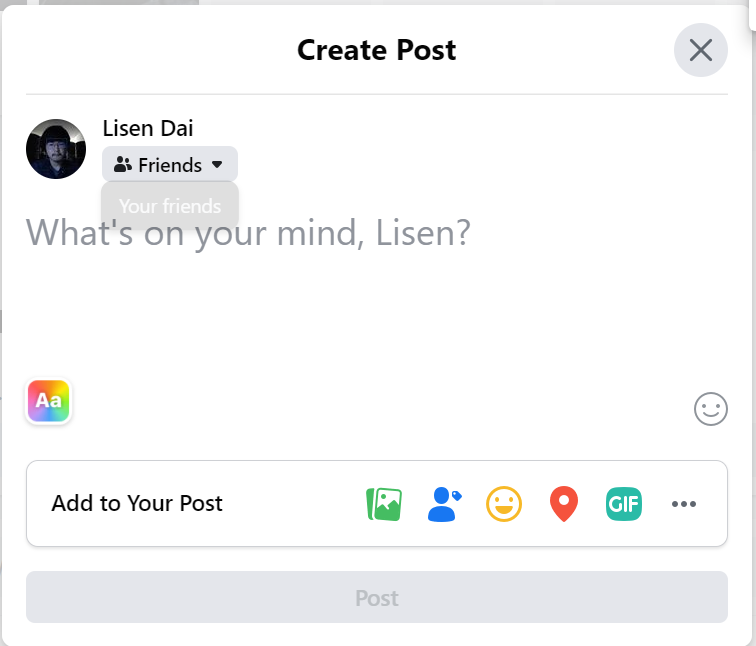
\includegraphics[scale=0.24]{src/img/Facebook.png} \\
                    \end{figure}

                    \begin{figure}[h]
                        \centering
                        
\includegraphics[scale=0.24]{src/img/Facebook_extension.png} \\
                    \end{figure}

                    \begin{figure}[h]
                        \centering
                        
\includegraphics[scale=0.24]{src/img/Tweet.png}
                    \end{figure}
                \end{column}
            \end{columns}
        \end{frame}
    
    \section*{任务概述}
        \begin{frame}
            \frametitle{任务结构}
            \begin{itemize}
                \item[-]{
                    API 接口设置
                    \begin{enumerate}
                        \item 利用社交媒体给出的接口,或者直接在网页上模拟人的交互,进行发帖操作。
                        \item 利用社交媒体给出的接口,或者利用爬虫等抓取方式,获取网络上的信息以供后端处理。
                    \end{enumerate}
                    \hspace*{\fill}\\
                    }
                \item[-]{
                    生成帖子
                    \begin{enumerate}
                        \item 利用已知\dotuline{信息}生成新的信息
                        \item 自动识别并且直接借用他人素材、链接,和现有的其他信息搭配
                    \end{enumerate}
                    } 
            \end{itemize}
        \end{frame}


        \begin{frame}
            \frametitle{API 接口简述}
            \begin{itemize}
                \item[-]{
                    发帖操作
                    \begin{enumerate}
                        \item 利用社交媒体给出的接口,或者直接在网页上模拟人的交互,进行发帖操作。
                        \item 利用社交媒体给出的接口,或者利用爬虫等抓取方式,获取网络上的信息以供后端处理。
                    \end{enumerate}
                    \hspace*{\fill}\\
                    }
                \item[-]{
                    生成帖子
                    \begin{enumerate}
                        \item 利用已知\textbf{信息}生成新的信息
                        \item 自动识别并且直接借用他人素材、链接,和现有的其他信息搭配
                    \end{enumerate}
                    } 
            \end{itemize}
        \end{frame}

        \begin{frame}
            \frametitle{信息生成}
            \begin{itemize}
                \item[-]{
                    发帖操作
                    \begin{enumerate}
                        \item 利用社交媒体给出的接口,或者直接在网页上模拟人的交互,进行发帖操作。
                        \item 利用社交媒体给出的接口,或者利用爬虫等抓取方式,获取网络上的信息以供后端处理。
                    \end{enumerate}
                    \hspace*{\fill}\\
                    }
                \item[-]{
                    生成帖子
                    \begin{enumerate}
                        \item 利用已知\textbf{信息}生成新的信息
                        \item 自动识别并且直接借用他人素材、链接,和现有的其他信息搭配
                    \end{enumerate}
                    } 
            \end{itemize}
        \end{frame}

        \begin{frame}
            \frametitle{信息生成}
            \begin{itemize}
                \item[-]{
                    发帖操作
                    \begin{enumerate}
                        \item 利用社交媒体给出的接口,或者直接在网页上模拟人的交互,进行发帖操作。
                        \item 利用社交媒体给出的接口,或者利用爬虫等抓取方式,获取网络上的信息以供后端处理。
                    \end{enumerate}
                    \hspace*{\fill}\\
                    }
                \item[-]{
                    生成帖子
                    \begin{enumerate}
                        \item 利用已知\textbf{信息}生成新的信息
                        \item 自动识别并且直接借用他人素材、链接,和现有的其他信息搭配
                    \end{enumerate}
                    } 
            \end{itemize}
        \end{frame}

        \begin{frame}
            \frametitle{信息生成}
            \begin{itemize}
                \item[-]{
                    发帖操作
                    \begin{enumerate}
                        \item 利用社交媒体给出的接口,或者直接在网页上模拟人的交互,进行发帖操作。
                        \item 利用社交媒体给出的接口,或者利用爬虫等抓取方式,获取网络上的信息以供后端处理。
                    \end{enumerate}
                    \hspace*{\fill}\\
                    }
                \item[-]{
                    生成帖子
                    \begin{enumerate}
                        \item 利用已知\textbf{信息}生成新的信息
                        \item 自动识别并且直接借用他人素材、链接,和现有的其他信息搭配
                    \end{enumerate}
                    } 
            \end{itemize}
        \end{frame}

\end{document}